\documentclass[tikz]{standalone}
\usepackage{tikz,amsmath}
\usetikzlibrary{calc}
\tikzstyle{vertex} = [draw, shape=circle, minimum width=.3cm, inner sep=.5pt]
\begin{document}
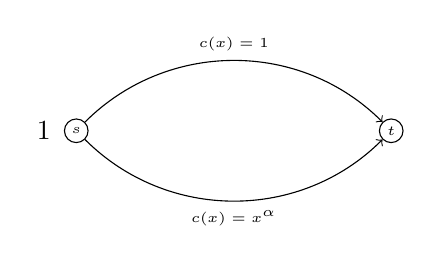
\begin{tikzpicture}[sloped]
    \draw (0,1) node[vertex] (s) {\tiny{$s$}};
    \draw (4,1) node[vertex] (t) {\tiny{$t$}};
    \draw (s) edge[out=45,in=135,->] node [above] {\tiny{$c(x)=1$}} (t);
    \draw (s) edge[out=-45,in=-135,->] node [below] {\tiny{$c(x)=x^\alpha$}} (t);
    \node at (s) [left=.2cm] {$\tiny{1}$};
\end{tikzpicture}
\end{document}
